\chapter{Architecture and design}
Requirements show what the system should do. \emph{Architecture and design} show \textbf{how} the system should be built. Architecture and design have the same flavour but they focus on different levels:
\begin{itemize}
\item Architecture stands at high level and handles decisions about major components and communication framework;
\item Design stands at lower level and handles decisions about internal structure of each component.
\end{itemize}
Most defects come from requirements and design, therefore it is essential to define, analyze and evaluate design choices early. If no design is defined, but code is immediately developed, choices are made implicitly and evaluate later. Doing design allows to make design choices \emph{explicit}, document and evaluate them. Given a set of requirements, in general, many different designs are possible corresponding to different design choices, but not all designs are equal. Transforming requirement to design is a creative process driven by skill and experience formalized in semi formal guidelines, i.e.\@ architectural styles (patterns) and design patterns.

Design has two sides:
\begin{itemize}
\item \textbf{System design}: decisions about computing nodes and their connection. For embedded systems it includes also decisions about components and connections in other technologies, i.e.\@ electrical, electronic, mechanical, etc.
\item \textbf{Software design}: decisions about software components and their connections, within a given system design.
\end{itemize}

\section{Process}
\begin{enumerate}
\item Architecture
\begin{itemize}
\item Define high level components and their interactions;
\item Select communication and coordination model
\item Use architectural styles or patterns;
\end{itemize}
\item Design
\begin{itemize}
\item High level, about many classes: define classes and their interactions using design patterns;
\item Lowe level, about one class.
\end{itemize}
\end{enumerate}

\subsection{Design}
Definition of classes can be done exploiting glossary or context diagram and considering design patterns.
From glossary, it is needed to consider a class for each key entity in glossary, while from context diagram it is needed to consider a class for each actor, i.e.\@ physical device or subsystem and define GUI for each human actor.

Low level design concerns a single class or two. For each attribute, define type and privacy. For each method, define return type, number and type of parameters, privacy and choose an algorithm if needed. Possibly define getters and setters. For each relationship with other class, choose an implementation. Persistence must be decided, too.

\paragraph{Relationship}
Relationships are not directly implemented in most programming languages. Representing a relationship is a design choice depending of the direction of the arrow, references, list, etc.

\section{Properties}
Properties are split in two categories:
\begin{itemize}
\item \textbf{Functional properties}: does the design support the functional requirements?
\item \textbf{Non functional properties}: does the design support the non functional properties?
\begin{itemize}
\item Reliability;
\item Efficiency/performance;
\item Usability;
\item Maintainability;
\item Portability;
\item Safety;
\item Security;
\end{itemize}
and some more specific to design:
\begin{itemize}
\item Testability (observability, controllability);
\item Monitorability;
\item Interoperability;
\item Scalability;
\item Deployability;
\item Mobility;
\item Complexity (number of components, number of interactions);
\item Coupling or decoupling (degree of dependence between two components);
\item Cohesion (degree of consistence of functions of a component);
\item Cost;
\item Schedule;
\item Staff skills.
\end{itemize}
\end{itemize}

\begin{description}
\item [Performance] Localize critical operation and minimize communications. Use large rather than fine-grain components.
\item [Security] Use a layered architecture with critical assets in the inner layers.
\item [Safety] Localize safety-critical features in a small number of sub-systems.
\item [Availability] Include redundant components and mechanism for fault tolerance.
\item [Maintainability] Use fine-grain, replaceable components.
\end{description}
Using large-grain components improves performance but reduces maintainability. Introducing redundant data improves availability but makes security more difficult. Localizing safety-related features usually means more communication, hence degraded performance.

\paragraph{Tradeoffs}
Not all properties can be satisfied. Design is also about deciding tradeoffs, which possibly are decided at requirement time.

\section{Notations for formalization of architecture}
\subsection{Informal}
\paragraph{Box and line diagrams}
Very abstract technique. Boxes and lines do not  show the nature of component relationships nor the externally visible properties of the subsystems. However, this technique is useful for communication with stakeholders and for project planning.

\subsection{Semiformal}
\paragraph{UML diagrams}
They provide a structural view of component:
\begin{itemize}
\item Component or package diagram for high level view;
\item Class diagram, inside each package or component;
\item Class description, for each class.
\end{itemize}
UML helps in presenting structure in an organized and hierarchical way. UML can provide a dynamic view, too by using sequence diagrams which represent the sequence in which functions are called, as shown in figure~\ref{sequence_diagram}.

\begin{figure}[hbtp]
\centering
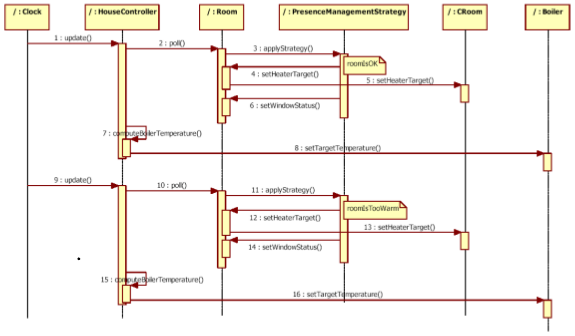
\includegraphics[scale=0.4]{images/uml_sequence_diagram.png}
\caption{Sequence diagram}
\label{sequence_diagram}
\end{figure}

\section{Patterns}
\emph{Patterns} are known and working ways of solving a problem. They provide reusable solutions to recurring problems in a defined context.

\subsection{Architectural patterns}
A real system is usually influenced by many architectural patterns.

\paragraph{Repository}
Subsystems must exchange data. When large amounts of data have to be shared, the repository model of sharing is the most commonly used. Sharing may be done in two ways:
\begin{itemize}
\item Shared data is held in a central database or repository and may be accessed by all subsystems;
\item Each subsystem maintains its own database and passes data explicitly to other subsystems.
\end{itemize}

\subparagraph{Advantages}
\begin{itemize}
\item Efficient way to share large amounts of data;
\item Subsystems need to be concerned with how data is produced;
\item Centralized management e.g.\@ backup, security;
\item Sharing model is published as the repository schema.
\end{itemize}

\subparagraph{Disadvantages}
\begin{itemize}
\item Subsystems must agree on a repository data model, which is inevitably a compromise;
\item Data evolution is difficult and expensive;
\item No scope for specific management policies;
\item Difficult to distribute efficiently.
\end{itemize}

\paragraph{Client-server model}
Distributed system model which shows how data and processing is distributed across a range of components. A set of stand-alone servers providing specific services can be accessed by a set of clients which can call these service, through a network which allows clients to access servers.

\subparagraph{Advantages}
\begin{itemize}
\item Distribution of data is straightforward;
\item Makes effective use of networked systems. May require cheaper hardware;
\item Easy to add new servers or upgrade existing servers.
\end{itemize}

\subparagraph{Disadvantages}
\begin{itemize}
\item No shared data model to subsystems using different data organization. Data interchange may be inefficient;
\item Redundant management in each server;
\item No central register of names and services. Finding out what servers and services are available may be hard.
\end{itemize}

\textbf{Abstract machine model} is used to model the interfacing of subsystems. It organizes the system into a set of layers, i.e.\@ abstract machines, each of which provide a set of services in such a way that a layer uses only services from adjacent layers.

In design, each layer is about a problem, i.e.\@ separation of concerns. In evolution, when a layer interface changes, only the adjacent layer is affected. The main problem is that sometimes is artificial to structure systems in this way.

\paragraph{Pipes \& Filters}
This technique is useful when data streams have to be processed according to several steps in a sequential way. It must be possible to recombine steps, taking into account that non-adjacent steps do not share any information and that the user storing data after each step may result into errors and garbage.

\paragraph{Other techniques}
Other possible techniques to use are layers, broker, MVC and microkernel.

%\subsection{Design patterns}
%\subsection{Idioms}

\section{Verification}
\emph{Verification} must check both functional and non functional requirements.

\subsection{Functional requirements}
\paragraph{Traceability matrix}
Each functional requirement must be supported by at least one function in one class in the software design. The more complex the requirement, the more member functions needed.

\paragraph{Scenarios}
Each scenario must be feasible. It is possible to define a sequence of calls to member functions of classes in the software design that matches the scenario.

\subsection{Non functional requirements}
Non functional requirements concern mostly of performance. Thus, scenarios are enriched with time model.

\subsection*{Bicycle example}
\paragraph{Functional requirements}
Transport one person from place to place.
\begin{itemize}
\item Steer;
\item Accelerate;
\item Brake.
\end{itemize}

\paragraph{Non functional requirements}
\begin{itemize}
\item Efficiency: speed from 10 km/h to 50 km/h, weight between 10 and 15 kg, reasonable torque to start (< 40 Nm);
\item Usability: out of 50 average users, at least 60\% of them find the bicycle easy to use;
\item Only human power, no engine;
\item Safety, no harm to driver;
\item Security, difficulty to steal;
\item Cost, between 100 and 200 euros.
\end{itemize}

\paragraph{Design vs requirements}
\begin{center}
\begin{tabularx}{\textwidth}{X|XXX}
 & Draisine & Velocipede & Dominant design \\ 
\hline 
Transport one person & Y & Y & Y \\ 
\hline 
Speed & < 10 km/h & Y & Y \\ 
\hline 
Torque at start & Y & N & Y \\ 
\hline 
Weight & Y & Y & Y \\ 
\hline 
Human power & Y & Y & Y \\ 
\hline 
Safety & Driver less high & Driver very high & Y \\ 
\hline 
Reduce speed & Feet on road & Negative force to pedal & Brakes \\ 
\end{tabularx}
\end{center}